\mychapter{Recursos avançados}\label{ch:metodosBasicos}

Este capítulo fornece uma visão mais detalhada do sistema MCTest, apresentado no capítulo anterior, destacando as funcionalidades específicas disponíveis para os três tipos de usuários: administrador, coordenador e professor. Cada um desses usuários tem acesso a um conjunto específico de funcionalidades para criar e gerenciar as diversas entidades do sistema, incluindo instituto, curso, disciplina, tópico e turma.

É relevante enfatizar que as entidades questão e exame serão discutidas em capítulos distintos nas Partes \ref{part:questoesMCTest} e \ref{part:exames} deste livro, respectivamente, devido à sua significativa importância no processo de avaliação. Nesta seção, serão abordadas as funcionalidades mais avançadas do MCTest disponíveis para cada tipo de usuário, visando facilitar a utilização efetiva do sistema.

Para fornecer exemplos práticos, serão criadas novas entidades no banco de dados disponibilizado no \href{https://github.com/fzampirolli/mctest}{GitHub}, apresentado na seção anterior. Essas entidades serão criadas de forma gradual e explicativa ao longo deste capítulo.

Cabe destacar que os usuários têm acesso somente às funcionalidades pertinentes ao seu papel no sistema. Por exemplo, um professor pode optar por estudar somente a Seção \ref{sec:professor} -- \nameref{sec:professor} deste capítulo para obter informações relevantes para as suas responsabilidades no MCTest.

\section{Administrador}

Nesta seção, serão discutidas outras funcionalidades destinadas ao administrador do sistema. O papel do administrador consiste em configurar o sistema conforme as necessidades da instituição, criar institutos, cursos e disciplinas necessários e disponibilizar as disciplinas aos coordenadores para poderem utilizá-las no sistema.

\subsection{Criar um curso relacionado a dois institutos}

No capítulo anterior, foi abordada a navegação individual de cada usuário na plataforma MCTest. Especificamente, nas Seções \ref{sec:instituto} -- \nameref{sec:instituto} e \ref{sec:curso} -- \nameref{sec:curso}, foi explorado como o administrador pode criar institutos e cursos, respectivamente. Em situações em que um curso é oferecido por dois institutos distintos, pode ser vantajoso configurar comportamentos específicos para cada um deles. Para ilustrar essa ideia, foi considerado hipoteticamente um curso de Engenharia da Computação na UFABC, dividido entre o Centro de Matemática, Computação e Cognição (CMCC) e o Centro de Engenharia, Modelagem e Ciências Sociais Aplicadas (CECS). Nesse contexto, seria interessante configurar o MCTest para permitir um acesso mais personalizado a cada instituto. Uma possível configuração para essa situação pode ser visualizada na Figura \ref{fig:cap03_instituicao2}, com a criação dos institutos CECS e CMCC.

Após o administrador clicar em ``Criar um novo Curso'' na Figura \ref{fig:cap03_figCursoListar2}, será exibida a tela de criação de um novo curso, apresentada na Figura \ref{fig:cap03_cursoCria2}. Para associar o curso a dois institutos distintos, basta manter o botão ``Ctrl'' pressionado e clicar nos institutos desejados. A tela de criação de um novo curso é semelhante à tela de atualização de um curso já existente. Observe na Figura \ref{fig:cap03_figCursoListar3} a lista de cursos vista pelo administrador após ter criado o curso de Engenharia da Computação na Figura \ref{fig:cap03_cursoCria2}. Na coluna ``Instituto'', o curso de Engenharia da Computação está associado aos centros CECS e CMCC.

\begin{figure}[!ht]
  \centering
  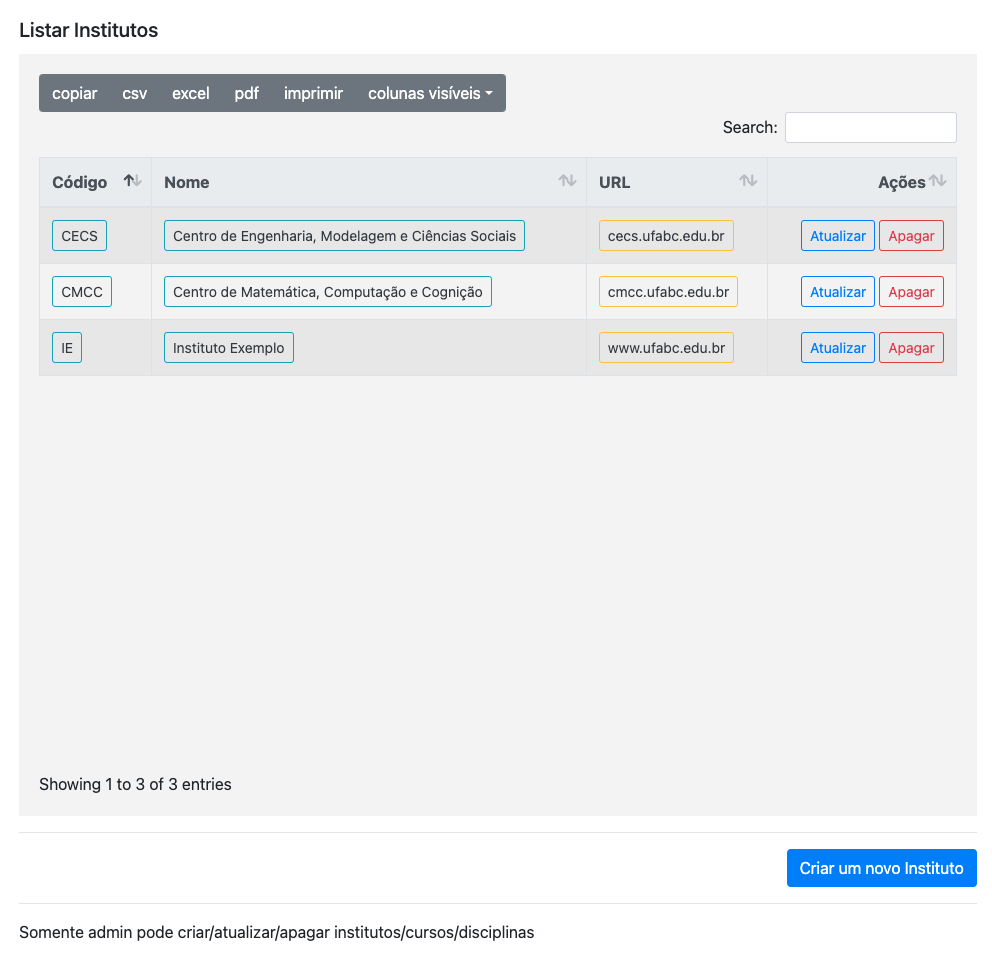
\includegraphics[width=0.9\textwidth]{cap03_figInstituto2.png}
  \caption{Tela com a lista de institutos vista pelo administrador, que pode atualizar, apagar ou criar um instituto para simular um curso pertencer aos institutos CECS e CMCC.}
  \label{fig:cap03_instituicao2}
\end{figure}

\begin{figure}[!ht]
  \centering
  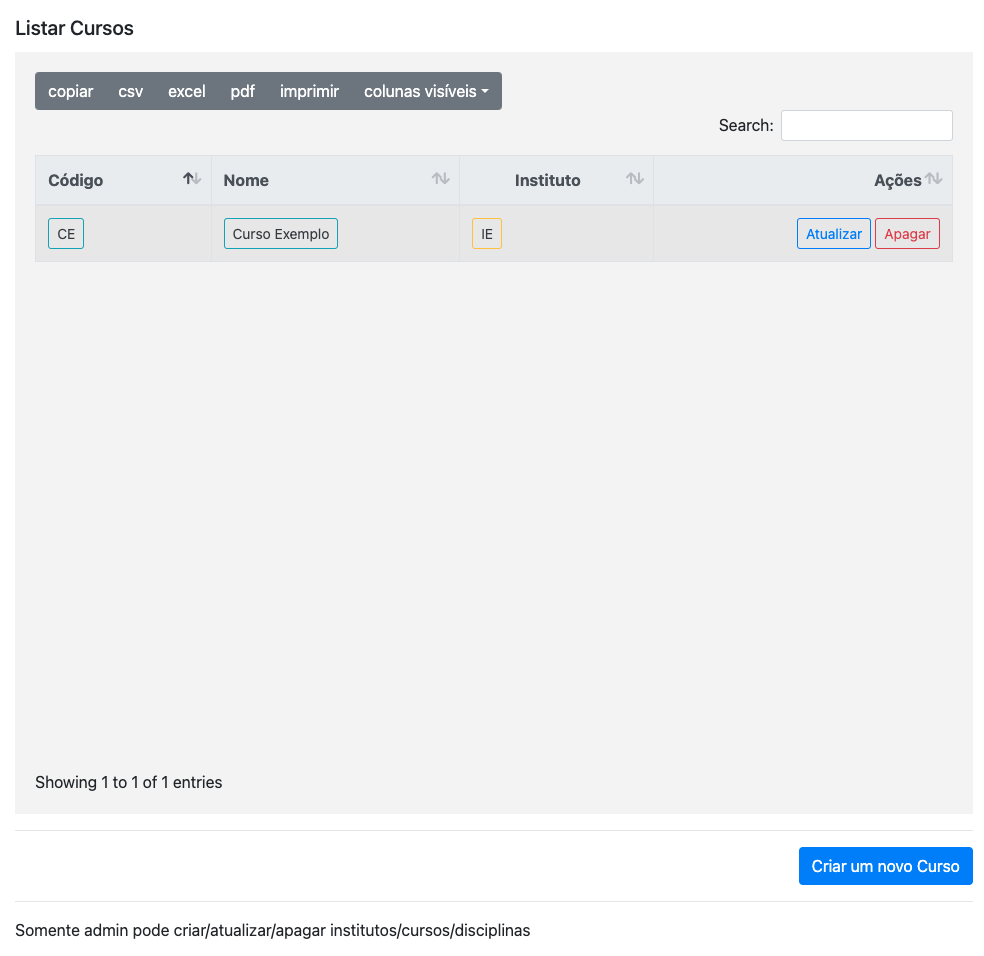
\includegraphics[width=0.9\textwidth]{cap03_figCursoListar2.png}
  \caption{Tela com a lista de curso, vista pelo administrador.}
  \label{fig:cap03_figCursoListar2}
\end{figure}

\begin{figure}[!ht]
  \centering
  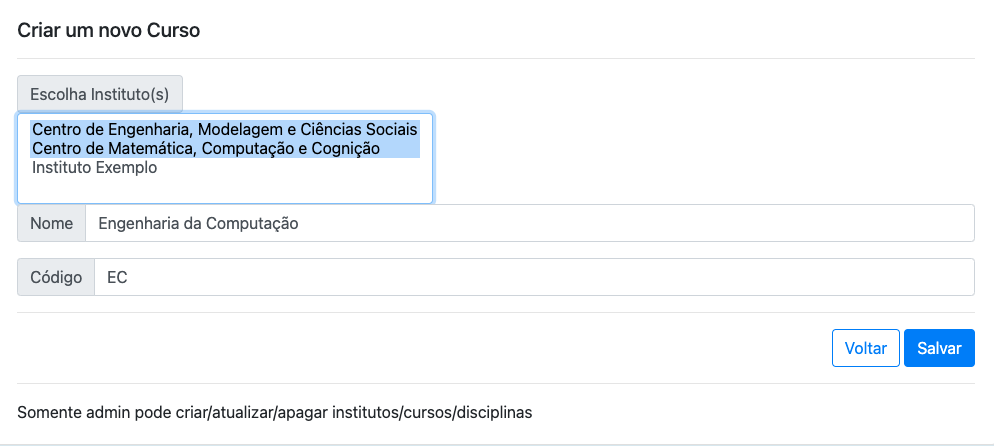
\includegraphics[width=0.9\textwidth]{cap03_figCursoCria2.png}
  \caption{Tela para o administrador criar um curso novo relacionado a dois institutos. Manter a tecla ``Ctrl'' pressionada para escolher mais de uma opção.}
  \label{fig:cap03_cursoCria2}
\end{figure}

\begin{figure}[!ht]
  \centering
  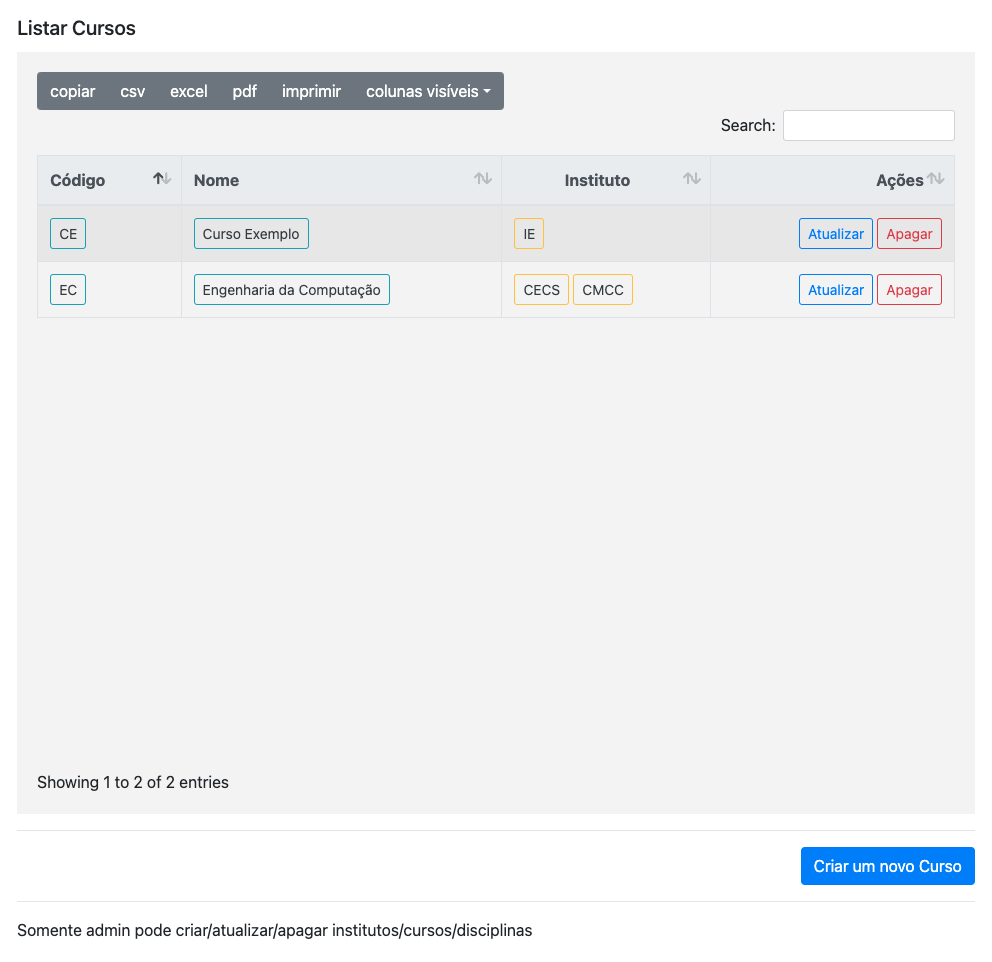
\includegraphics[width=0.9\textwidth]{cap03_figCursoListar3.png}
  \caption{Tela com a lista de curso, vista pelo  administrador, após ter criado o curso Engenharia da Computação na Figura \ref{fig:cap03_cursoCria2}.}
  \label{fig:cap03_figCursoListar3}
\end{figure}

\subsection{Criar uma disciplina relacionada a dois cursos}

Nas Seções \ref{sec:curso} -- \nameref{sec:curso} e \ref{sec:disciplina} -- \nameref{sec:disciplina}, foram abordados os procedimentos para o administrador poder criar cursos e disciplinas, respectivamente. Para ilustrar a relevância da criação de uma disciplina relacionada a dois cursos, será apresentado o seguinte cenário.

A disciplina de Processamento Digital de Imagens (PDI) é uma área da Ciência da Computação que se dedica ao estudo e desenvolvimento de técnicas e algoritmos para manipulação, análise e PDI. Essa disciplina é muito importante tanto para estudantes de graduação em Ciência da Computação quanto para estudantes de mestrado e doutorado, por oferecer uma base sólida de conhecimentos e habilidades para a solução de problemas em diversas áreas de aplicação.

No curso de graduação em Ciência da Computação, a disciplina de PDI aborda diversas técnicas relevantes para o processamento e análise de imagens digitais. Entre elas, destaca-se a representação de imagens digitais, que envolve o uso de matrizes para representar as cores dos pixels, e técnicas de filtragem, que permitem a melhoria da qualidade da imagem, através da redução de ruídos e realce de contornos de objetos.

Além disso, a disciplina de PDI também aborda técnicas de segmentação de imagens, que permitem a identificação de regiões de interesse na imagem, e técnicas de reconhecimento de padrões em imagens, que permitem a identificação de objetos, faces e outros elementos na imagem.

Durante o curso de mestrado ou doutorado em Ciência da Computação, a disciplina de PDI explora técnicas avançadas, incluindo o uso de Redes Neurais Convolucionais (CNN -- do inglês \textit{Convolutional Neural Network}). Essas técnicas têm se mostrado altamente eficazes para a segmentação, reconhecimento e classificação de imagens.

As CNN são uma classe de Redes Neurais Artificiais que têm sido amplamente utilizadas em tarefas de PDI, como a segmentação de objetos em imagens médicas ou a classificação de imagens em categorias específicas. Essas redes podem extrair características das imagens de forma automática, sem a necessidade de recursos humanos para a extração manual de características.

Com a utilização de CNN, é possível obter excelentes resultados na segmentação, reconhecimento e classificação de imagens. Por exemplo, na área médica, é possível identificar automaticamente regiões de interesse em imagens de ressonância magnética ou tomografia computadorizada, auxiliando no diagnóstico de doenças.

Portanto, a disciplina de PDI é de grande importância tanto para os estudantes de graduação quanto para os estudantes de mestrado e doutorado em Ciência da Computação. Além disso, as questões relacionadas a essa disciplina podem ser compartilhadas entre esses dois cursos.

Dessa forma, é viável adicionar a disciplina de PDI no MCTest e relacioná-la com os cursos de graduação e pós-graduação, conforme ilustrado na Figura \ref{fig:cap03_figDisciplina2}. Esse processo é semelhante ao de associar um curso a dois institutos.

\begin{figure}[!ht]
  \centering
  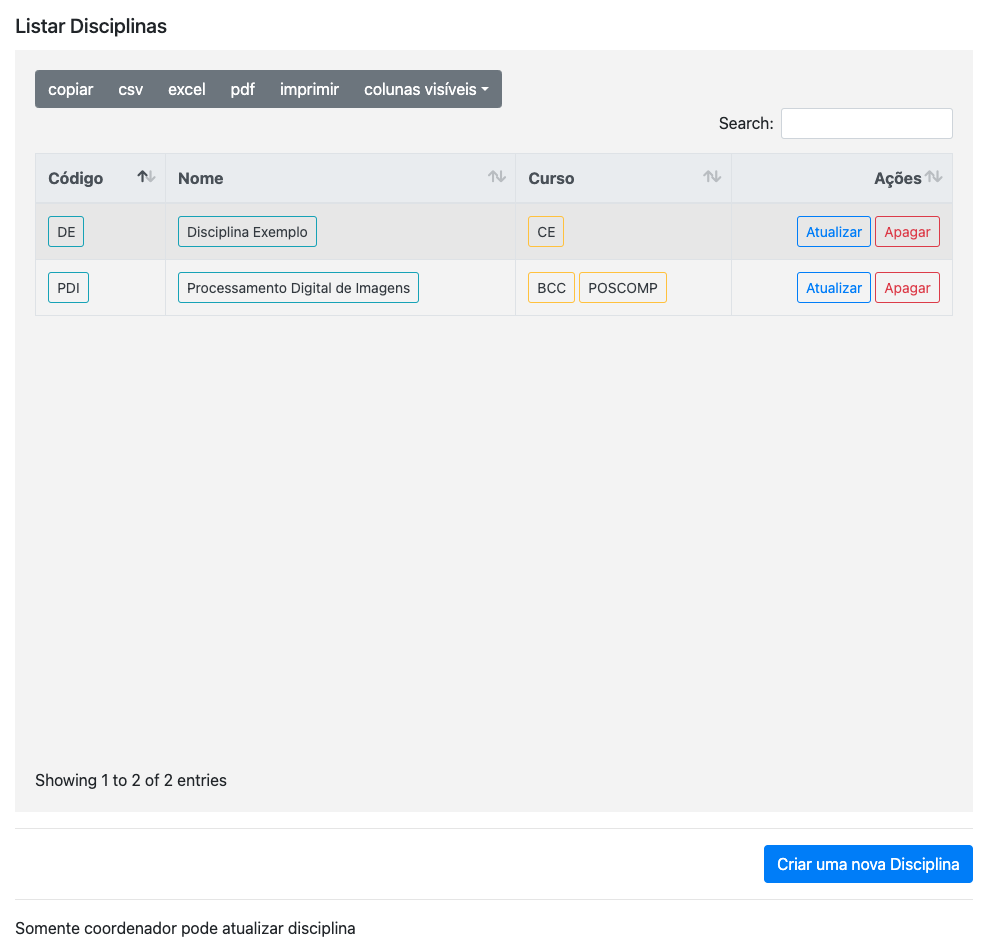
\includegraphics[width=0.9\textwidth]{cap03_figDisciplina2.png}
  \caption{Tela com a lista de disciplinas, vista pelo  administrador, com destaque para a disciplina PDI, que está relacionada aos cursos de BCC e POSCOMP.}
  \label{fig:cap03_figDisciplina2}
\end{figure}

\subsection{Acesso ao banco de dados}

Embora o administrador tenha acesso direto ao banco de dados (BD) ao pressionar o botão ``Admin'' na Figura \ref{fig:cap2_navegacao}-(e), a melhor opção é evitar alterar o BD usando esse recurso. É recomendado utilizar as telas de navegação do MCTest para fazer as alterações necessárias, pois alterar o BD diretamente pode resultar em relacionamentos incorretos entre as entidades, o que pode tornar o sistema inoperante. %Para aqueles que desejam obter detalhes sobre a arquitetura de software e o banco de dados desenvolvido no MCTest, recomendamos consultar a Parte \ref{part:topicosAvancados} deste livro.

\begin{figure}[!ht]
  \centering
  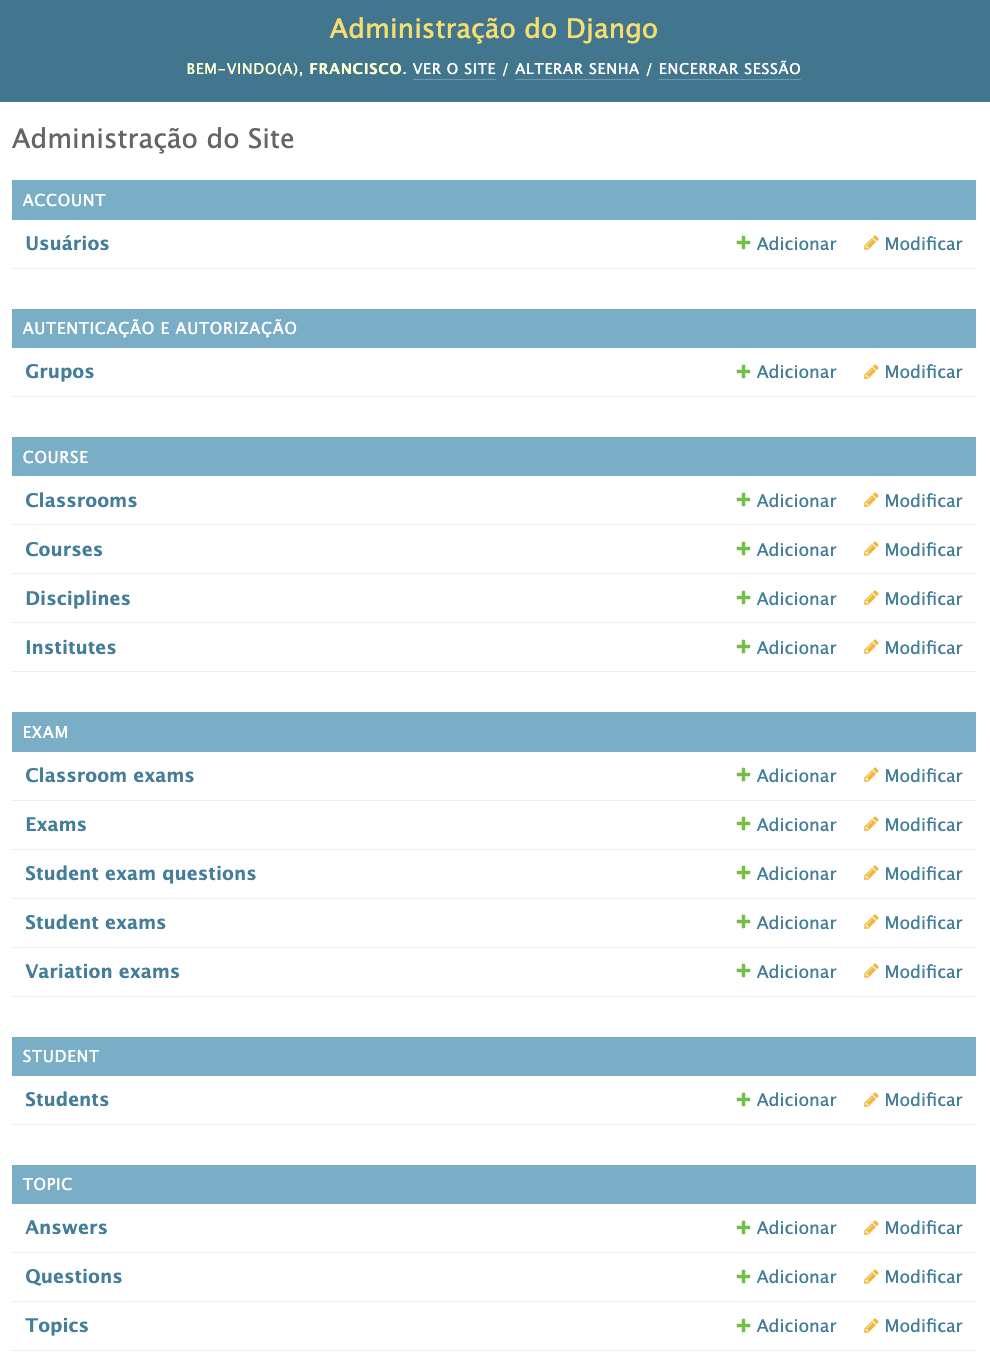
\includegraphics[width=0.85\textwidth]{cap03_figAdminBD.png}
  \caption{Tela com a lista de entidades que o administrador pode fazer manutenção diretamente no BD.}
  \label{fig:cap03_figAdminBD}
\end{figure}


\section{Coordenador}

Nesta seção, serão abordadas as funcionalidades destinadas ao coordenador de disciplina, que envolvem a manutenção de tópicos e disciplinas. O coordenador tem a responsabilidade de criar e gerenciar os tópicos e disciplinas que serão utilizados pelos professores para criar exames e Exercícios de Programação (EPs).

\subsection{Criar um tópico relacionado a duas ou mais disciplinas}

A interdisciplinaridade é uma abordagem essencial na educação moderna, que visa integrar conhecimentos de diferentes áreas para enriquecer o processo de aprendizagem e formação dos estudantes. Nesse sentido, a UFABC se destaca na interdisciplinaridade, conforme apresentado em sua missão:

\begin{mybox}{green}{\textbf{Missão da UFABC:\\\vspace{-3mm}\hrule}}
\begin{quote}
    \textit{Promover o avanço do conhecimento por ações de ensino, pesquisa e extensão, tendo como fundamentos básicos a interdisciplinaridade, a excelência e a inclusão social.}
\end{quote}
\end{mybox}

Nesse sentido, compartilhar um tópico entre duas ou mais disciplinas pode trazer inúmeros benefícios para a educação. Como mencionado na Seção \ref{sec:topicos} -- \nameref{sec:topicos}, um tópico só existe no MCTest se pertencer a uma disciplina, mas pode ser compartilhado entre várias delas. Além disso, as questões só existem se estiverem inseridas em um tópico. 


Um exemplo prático dessa abordagem pode ser observado na UFABC, onde a lógica de programação é abordada em diversas disciplinas. Especificamente, esse tópico é tratado no Bacharelado em Ciência e Tecnologia (BCT), no segundo exame da disciplina de Bases Computacionais da Ciência (CS0) para os ingressantes e também no primeiro exame de Processamento da Informação (PI -- CS1) no terceiro quadrimestre dos ingressantes. Atualmente, a maioria das turmas dessas duas disciplinas utiliza a linguagem Python. Além disso, a disciplina de Programação Estruturada (PE -- CS2) do Bacharelado em Ciência da Computação também aborda a lógica de programação no primeiro exame, utilizando a linguagem C.

Ao elaborar questões sobre lógica de programação de forma independente da linguagem utilizada, é possível compartilhar essas questões entre as três disciplinas mencionadas. Essa prática tem várias vantagens:

\begin{description}
\item[Otimização de recursos:] Ao compartilhar questões e tópicos, é possível economizar tempo e esforço dos professores na criação de materiais didáticos, permitindo que se concentrem em outras tarefas importantes, como atendimento aos estudantes e pesquisas de novas metodologias de ensino;

\item[Consistência no conteúdo:] Ao utilizar tópicos comuns entre diferentes disciplinas, os estudantes são expostos a uma abordagem consistente e coerente, facilitando a compreensão e a conexão entre os conceitos aprendidos;

\item[Desenvolvimento de habilidades transferíveis:] Ao aprender sobre um tópico em várias disciplinas, os estudantes têm a oportunidade de desenvolver habilidades transferíveis, como pensamento crítico, resolução de problemas e comunicação. Essas habilidades são essenciais para o sucesso em diversas áreas profissionais;

\item[Fomento da interdisciplinaridade:] Compartilhar tópicos entre disciplinas incentiva os estudantes a estabelecer conexões entre diferentes campos do conhecimento, promovendo uma educação mais integrada e abrangente.
\end{description}

A Figura \ref{fig:cap03_figTopico2} exemplifica uma lista de tópicos, demonstrando que um determinado tópico pode pertencer a três disciplinas diferentes. Adicionalmente, a Figura \ref{fig:cap03_figDisciplina3} apresenta detalhes específicos da disciplina de Processamento da Informação, com destaque para os tópicos compartilhados. Essa configuração permite que um professor utilize todas as questões desses tópicos ao elaborar um exame.

\begin{figure}[!ht]
  \centering
  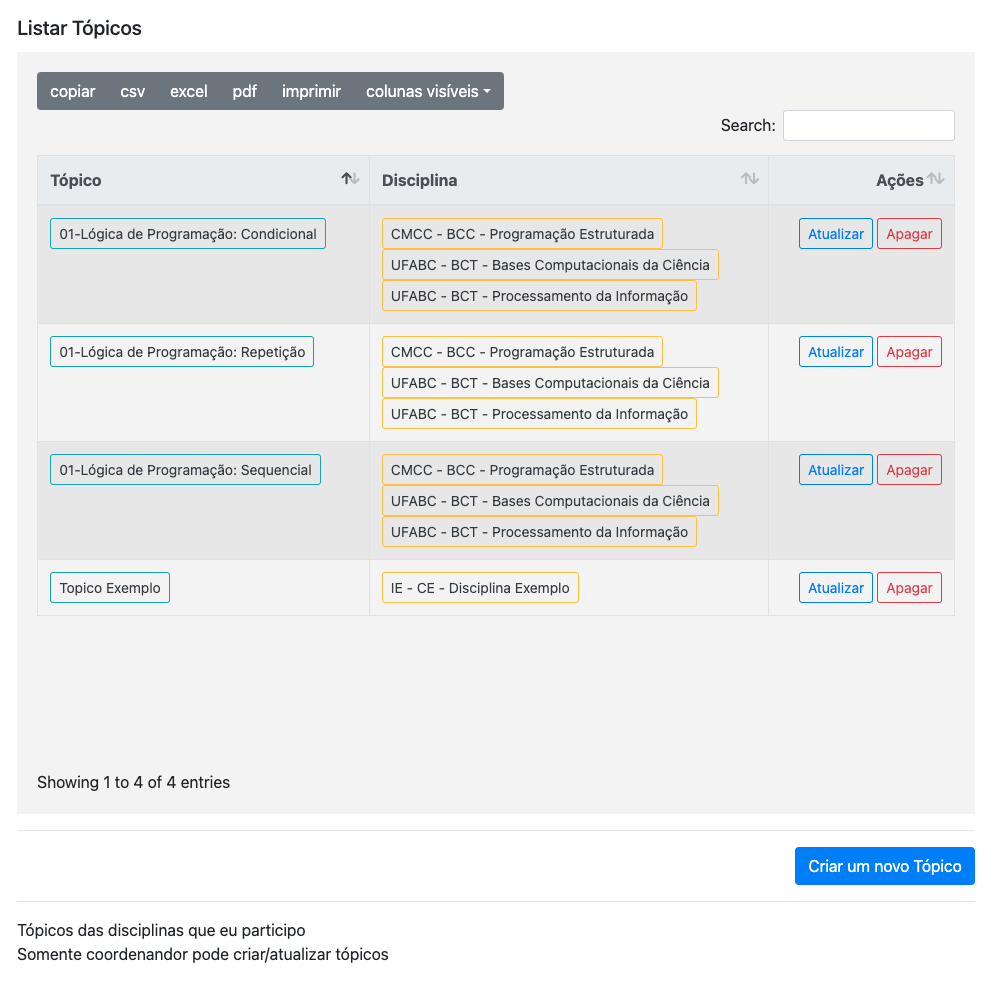
\includegraphics[width=0.9\textwidth]{cap03_figTopico2.png}
  \caption{Tela com a lista de tópicos, vista pelo  coordenador. É possível observar o compartilhamento de tópicos entre disciplinas.}
  \label{fig:cap03_figTopico2}
\end{figure}

\begin{figure}[!ht]
  \centering
  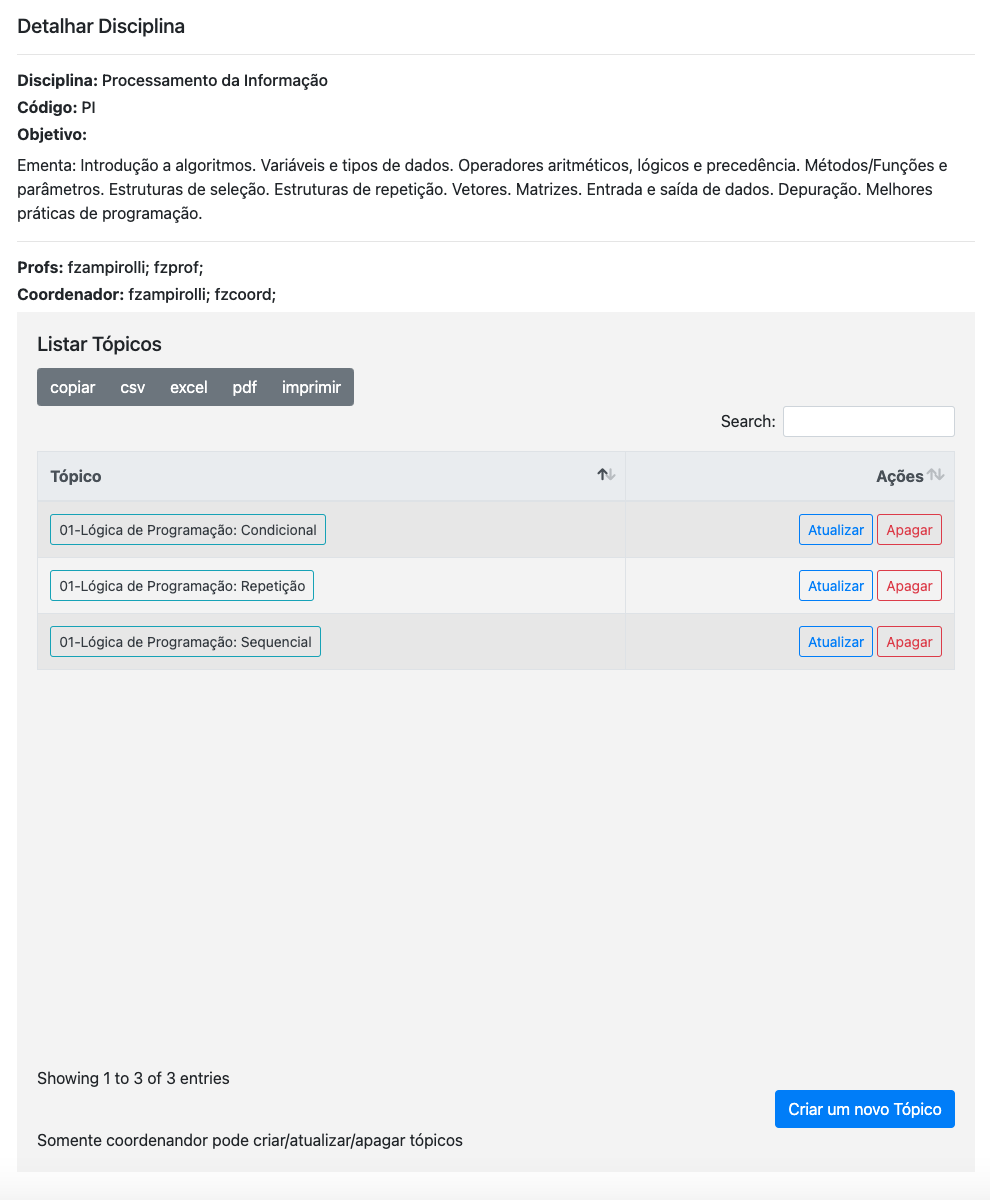
\includegraphics[width=0.9\textwidth]{cap03_figDisciplina3.png}
  \caption{Tela com detalhes da disciplina de Processamento da Informação, vista pelo  coordenador, com os tópicos compartilhados também apresentados na Figura \ref{fig:cap03_figTopico2}.}
  \label{fig:cap03_figDisciplina3}
\end{figure}


\subsection{Criar várias turmas com arquivo CSV}\label{sec:variasTurmasCSV}

No capítulo anterior, foi abordada a criação de disciplinas na Seção \ref{sec:disciplina} -- \nameref{sec:disciplina}, e a criação de turmas com estudantes foi apresentada na Seção \ref{sec:turma} -- \nameref{sec:turma}. No entanto, em algumas situações, pode ser necessário criar várias turmas da mesma disciplina simultaneamente. Para atender a essa demanda, foram implementadas funcionalidades que permitem ao coordenador cadastrar todos os professores e estudantes de múltiplas turmas de uma só vez, por meio da importação de arquivos no formato CSV, conforme ilustrado na Figura \ref{fig:cap03_figDisciplinaAtualiza22}.

\begin{mybox}{pink}{\textbf{Melhorias:\\\vspace{-3mm}\hrule\vspace{3mm}}}
É importante ressaltar que esse recurso precisa ser aprimorado e, por enquanto, o botão ``Upload-Turma'' irá remover todos os estudantes de todas as turmas associadas a essa disciplina, atualizando com os novos dados do arquivo CSV. Portanto, é fundamental ter cuidado ao utilizar essa funcionalidade e garantir que os dados do arquivo CSV estejam corretos e atualizados.
\end{mybox}

%Essa funcionalidade é extremamente útil para facilitar o cadastro de muitos estudantes e professores de uma só vez, além de permitir que os dados sejam atualizados de forma mais eficiente. No entanto, é importante lembrar que a precisão e a consistência dos dados do arquivo CSV são fundamentais para a realização de exames precisos e eficazes.

\begin{figure}[!ht]
  \centering
  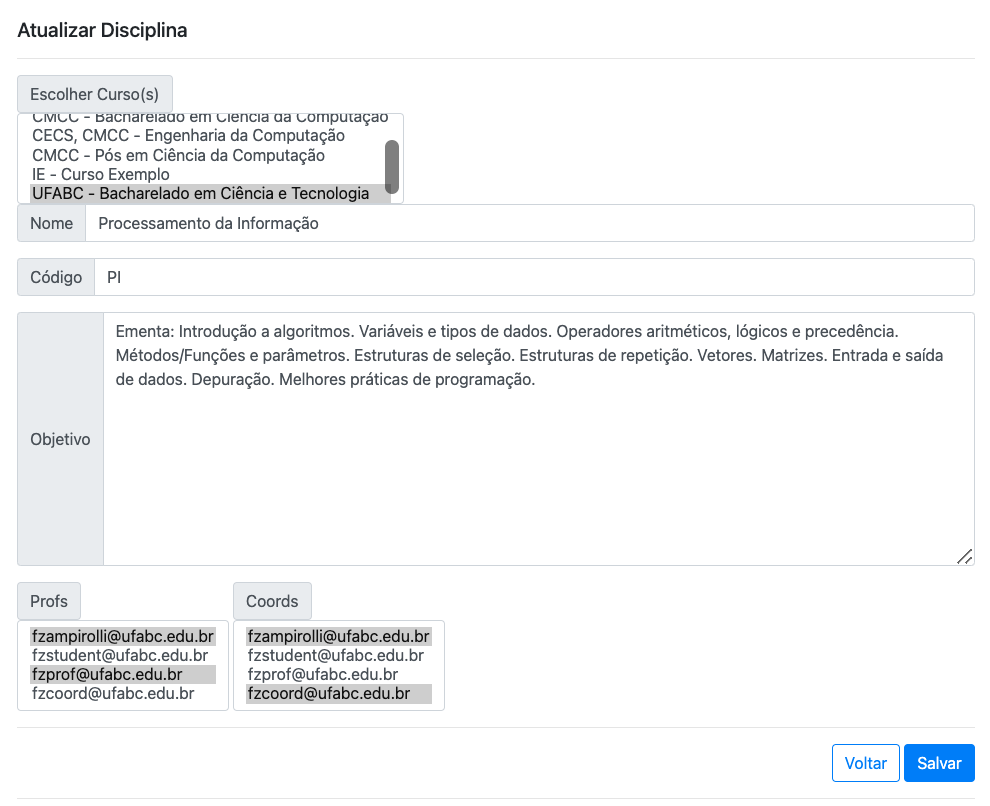
\includegraphics[width=0.9\textwidth]{cap03_figDisciplinaAtualiza2a.png}
  \caption{(Parte 1) Tela de criação da disciplina de Processamento da Informação pelo administrador.}
  \label{fig:cap03_figDisciplinaAtualiza2a}
\end{figure}

\begin{figure}[!ht]
  \centering
  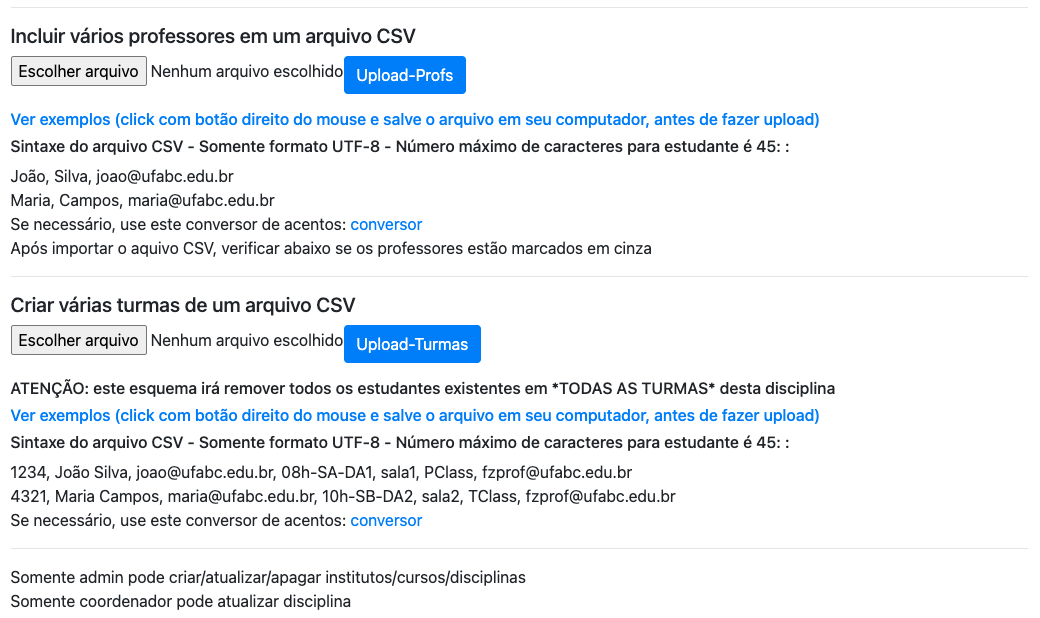
\includegraphics[width=0.9\textwidth]{cap03_figDisciplinaAtualiza22.png}
  \caption{(Parte 2) Tela de criação da disciplina de Processamento da Informação pelo administrador. É possível incluir professores, turmas e estudantes pela importação de dois arquivos no formato CSV.}
  \label{fig:cap03_figDisciplinaAtualiza22}
\end{figure}

As telas para criação e atualização de disciplinas apresentadas nas Figuras \ref{fig:cap03_figDisciplinaAtualiza2a} e \ref{fig:cap03_figDisciplinaAtualiza22} são semelhantes e estão disponíveis tanto para o administrador quanto para o coordenador da disciplina. 
Na Figura \ref{fig:cap03_figDisciplinaAtualiza22}, o primeiro arquivo CSV é destinado ao coordenador para inserir diversos professores na disciplina, com o perfil de professor já configurado, como apresentado a seguir:
\begin{myboxCode}{corCSV}{\textbf{Arquivo CSV com dados dos professores:}}\vspace{3mm}
\hrule
\begin{verbatim}
123, João da Silva, joao@ufabc.edu.br
987, Maria Gonçalves, maria@ufabc.edu.br
\end{verbatim}
\end{myboxCode}

Por sua vez, o segundo arquivo CSV nesta figura é utilizado pelo coordenador para adicionar várias turmas, contendo estudantes e professores, com um formato pré-definido como segue:
\begin{myboxCode}{corCSV}{\textbf{Arquivo CSV com dados de estudantes e professores:}}\vspace{3mm}
\hrule
\begin{verbatim}
123, João Silva, js@gmail.com, DA1, sala1, PClass, fzprof@ufabc.edu.br
987, Maria Campos, mc@gmail.com, DA2, sala2, TClass, fzprof@ufabc.edu.br
\end{verbatim}
\end{myboxCode}

Este último arquivo CSV apresenta as seguintes colunas, em ordem: identificação do estudante, nome completo do estudante, e-mail do estudante, turma, sala, ``PClass'' (para turma prática) ou ``TClass'' (para turma teórica) e e-mail do professor.


\section{Professor} \label{sec:professor}

Nesta seção será abordada mais funcionalidades destinadas aos professores, que incluem a manutenção de turmas, questões e exames. O professor é responsável por criar as turmas, selecionar as questões e criar os exames para avaliar os estudantes. Com o sistema MCTest, os professores podem criar exames com questões de múltipla escolha (QMs) ou dissertativas (QTs), incluindo EPs parametrizados para correção automática no Moodle, utilizando o \textit{plugin} VPL.

\subsection{Criar turma com arquivo CSV}\label{sec:professorCriarTurma}

O professor é responsável por criar uma turma e manter os dados de seus estudantes atualizados, como discutido na Seção \ref{sec:turma} -- \nameref{sec:turma}. O primeiro passo é criar a turma e relacioná-la a uma disciplina, conforme ilustrado na Figura \ref{fig:cap02_figTurmaCriar}. Em seguida, o professor pode inserir os estudantes de três maneiras distintas:

\begin{enumerate}
    \item  Selecionando vários estudantes na lista com a tecla ``Ctrl'' pressionada, como demonstrado na Figura \ref{fig:cap02_figTurmaAtualiza};
    \item Incluindo um estudante de cada vez, conforme exemplificado na Figura \ref{fig:cap02_figTurmaAtualiza2} e/ou atualizando os dados de um estudante, como demonstrado na Figura \ref{fig:cap02_figTurmaAtualiza3}; 
    \item Ou, de maneira mais eficiente, utilizando um arquivo CSV, vistos a seguir.
\end{enumerate}

Para utilizar um arquivo CSV para preencher uma turma com estudantes, o professor deve primeiro criar a turma, como ilustrado na Figura \ref{fig:cap02_figTurmaCriar}, e em seguida fazer o \textit{upload} do arquivo no início da Figura \ref{fig:cap02_figTurmaAtualiza}, selecionando o arquivo em ``Escolher arquivo'' e, em seguida, clicando no botão ``Importar-Estudantes''. O arquivo deve seguir o formato apresentado abaixo:

\begin{myboxCode}{corCSV}{\textbf{Arquivo CSV com dados completos:}}\vspace{3mm}
\hrule
\begin{verbatim}
123, João da Silva, joao@aluno.ufabc.edu.br
987, Maria Gonçalves, maria@aluno.ufabc.edu.br
\end{verbatim}
\end{myboxCode}

Observe que a primeira linha do arquivo já representa o primeiro estudante, com sua identificação, nome completo e e-mail, separados por vírgula ou ponto e vírgula. É importante destacar que o e-mail é opcional, como no exemplo abaixo:

\begin{myboxCode}{corCSV}{\textbf{Arquivo CSV, sem e-mail: }}\vspace{3mm}
\hrule
\begin{verbatim}
123, João da Silva
987, Maria Gonçalves
\end{verbatim}
\end{myboxCode}

\subsection{Criar turma com arquivo CSV -- restrições}\label{sec:professorCriarTurma2}

O professor deve ter uma atenção especial aos acentos e símbolos especiais neste arquivo CSV, que deve seguir o formato \texttt{UTF-8}. Uma alternativa é converter esses símbolos para o formato \LaTeX{}, utilizando, por exemplo, o recurso disponível na internet em \href{https://w2.syronex.com/jmr/latex-symbols-converter}{w2.syronex.com/jmr/latex-symbols-converter}, conforme exemplo abaixo:

\begin{myboxCode}{corCSV}{\textbf{Arquivo CSV, com acentos no formato \LaTeX: }}\vspace{3mm}
\hrule
\begin{verbatim}
123, Jo\~{a}o da Silva, joao@aluno.ufabc.edu.br
987, Maria Gon\c{c}alves, maria@aluno.ufabc.edu.br
\end{verbatim}
\end{myboxCode}

\begin{mybox}{corObs}{\textbf{Observações:\\\vspace{-3mm}\hrule\vspace{1mm}}}
\begin{enumerate}
    \item O nome do estudante no sistema tem um limite de 45 caracteres. Caso o arquivo CSV contenha um nome de estudante com mais de 45 caracteres, o sistema irá remover automaticamente o(s) sobrenome(s) do meio, de trás para frente, mantendo o último sobrenome, até atingir os 45 caracteres permitidos. Essa medida é tomada para garantir a integridade dos dados e evitar problemas de exceder o limite de caracteres ao incluir o nome do estudante em um exame. Um exemplo pode ser visto na Figura \ref{fig:cap03_figTurmaCSV};
    \item Caso o arquivo contenha um identificador já existente, o sistema não criará ou alterará o mesmo.
\end{enumerate}
\end{mybox}

\begin{figure}[!ht]
  \centering
  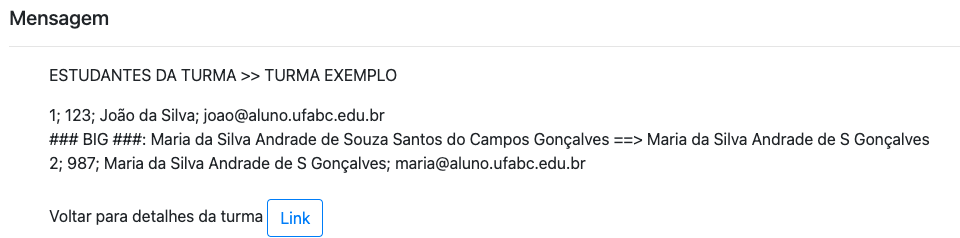
\includegraphics[width=0.9\textwidth]{cap03_figTurmaCSV.png}
  \caption{Tela mostrando o resultado do cadastro de estudantes utilizando a importação de um arquivo no formato CSV.}
  \label{fig:cap03_figTurmaCSV}
\end{figure}

\section{Considerações finais}

Este capítulo expandiu as funcionalidades apresentadas no capítulo anterior, apresentando recursos avançados disponíveis no MCTest para usuários com diferentes papéis (administrador, coordenador e professor). Cada tipo de usuário tem acesso a um conjunto específico de ferramentas para criar e gerenciar as diversas entidades do sistema de avaliação, como institutos, cursos, disciplinas, tópicos, turmas, professores e estudantes.

As funcionalidades abordadas procuram facilitar o gerenciamento das entidades e a configuração do sistema conforme as necessidades de cada instituição. O administrador, em particular, tem permissões amplas para configurar o sistema e gerenciar o acesso dos usuários. Os coordenadores são responsáveis por gerenciar disciplinas, tópicos e turmas. Já os professores podem gerenciar questões, exames, turmas e estudantes sob sua responsabilidade.

Nos próximos capítulos da Parte \ref{part:questoesMCTest}, serão abordados a criação e o gerenciamento de questões no MCTest, com foco nas diversas formas de elaboração, revisão e aprovação das questões destinadas a serem aplicadas nos exames discutidos na Parte \ref{part:exames}.